\documentclass[class=article, crop=false, 12pt]{standalone}
\usepackage[subpreambles=true]{standalone}
\usepackage{../.common/common}


\author{Tony Shing}
%\pretitle{Supplementary}

\topic{T12 (Electromagnetism)}
\title{Magnetostatics}

\version{2025} % leave blank for omitting

\begin{document}

\maketitle


\begin{overview}
    \begin{itemize}
        \item Basic problems: Find $\vvec{B}$ by Biot-Savat law with integration
        \item Divergent-less of B-field
        \item Ampere's law, dot product line integral, curl \& Stokes' theorem
        \item \it{(Optional reading)} Magnetic vector potential \& Poisson equation
    \end{itemize}


\end{overview}

\vskip 1em
In electromagnetism, 
theoretically every problem can be solved through a set of PDEs
called the \bf{Maxwell Equations}.\\[-2em]
\begin{center}
    \begin{minipage}{0.3\textwidth}
        \aleq{
            {\div} \vvec{E} &= \frac{\rho}{\epsilon_0}\\
            \curl \vvec{E} &= -\pdvv{\vvec{B}}{t}
        }
    \end{minipage}
    \hspace{0.05\textwidth}
    \begin{minipage}{0.3\textwidth}
        \aleq{
            \tkn{maxwell_div}{\div} \vvec{B} &= 0\\
            \tkn{maxwell_ampere}{\curl} \vvec{B} &= \mu_0 \vvec{J} + \mu_0\epsilon_0\pdvv{\vvec{E}}{t}
        }
    \end{minipage}
\end{center}
\addArrow[blue]{maxwell_div}{(-5ex,0)}{}{(-3ex,1ex)}
\addArrow[red]{maxwell_ampere}{(-5ex,0)}{}{(-3ex,1ex)}

However, a \it{system of PDEs} is too complicated to be solved.
So we need to learn different "tricks" to avoid them,
which are enough for some simple scenarios.\\

Magnetostatics only concerns the \nth{2} and \nth{4} equation of the set 
- \cul[blue]{Gauss's law on B-field} and \cul[red]{Ampere's law}. 




\linesep
% content begins here
% Section %%%%%%%%%%%%%%%%%%%%%%%%%%%%%%%%%%%%%%%%%%%%%%%%%%%%
\section{Basic Skill: Biot-Savat Law with Integration}

Physically, currents are just moving charges. 
There is no such thing called "point current".
However we can imagine a line of current being divided into many infinitestimally small segments
such that each current segment "looks like" a vector point source.
\aleq{
    \ \ \qty(\mstack{\text{Current}\\\text{line}}) \ =\ I\vvec{L} 
    \quad\ \xRightarrow{\phantom{000}}\quad\ \ 
    \int I \dd{\vvec{l}} \ \sim\ \sum \qty(\mstack{\text{Current}})\qty(\mstack{\text{Unit}\\\text{length}})
}

\begin{center}
    \begin{minipage}{0.3\linewidth}
        \centering
        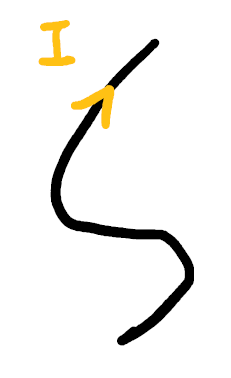
\includegraphics[height=10em]{current_line1}
    \end{minipage}
    {\Large \qquad$\Rightarrow$\qquad}
    \begin{minipage}{0.3\linewidth}
        \centering
        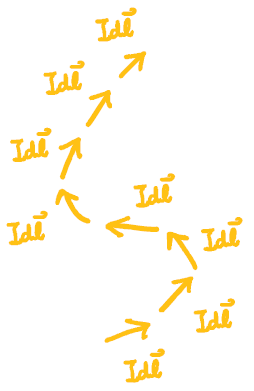
\includegraphics[height=10em]{current_line2}
    \end{minipage}
\end{center}

In reality, current sources must form a continuous line and 
cannot suddenly appear / disappear at nowhere.
This is why Biot-Savat law must be written as an integral and so
never be found in your high school textbooks.
\aleq{
    \cus[red]{\vvec{B} = \frac{\mu_0}{4\pi} \frac{I\vvec{L}}{r^2}\cross \hhat{r}}
        {\substack{\text{Always remember that}\\\text{You should not write this}}}
    \qquad\xRightarrow{\phantom{000}}\quad
    \cus[blue]{\int \dd{\vvec{B}} 
    = \int_{\substack{\text{whole}\\\text{line}}} \frac{\mu_0}{4\pi} \frac{I\dd{\vvec{l}}}{r^2}\cross\hhat{r}}
        {\substack{\text{Biot-Savat law can only be}\\\text{written as an integral}}}
}

Furthermore, because we are living in a 3D world,
current does not always travel along a line segment, 
but may flow on a surface or through an object such that the current is position dependent. 
In these cases, we should describe current as a distribution of flow (i.e. vector field).


\begin{center}
    \vskip 1em
    \begin{minipage}{0.45\linewidth}
        \centering
        When current is travelling on a surface, 
        the current flow is described as a 2D vector field called \bf{surface current density} $\vvec{K}$. 
        \aleq{
            I\dd{\vvec{l}} 
            \qquad\xRightarrow{\phantom{0}}\quad 
            \vvec{K}\dd{s}
        }
        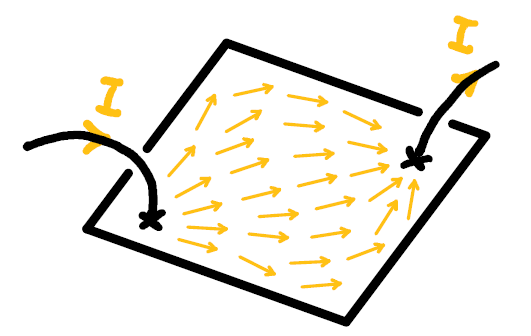
\includegraphics[height=8em]{current_sur}
    \end{minipage}
    \hspace{0.02\textwidth}
    \vline
    \hspace{0.02\textwidth}
    \begin{minipage}{0.45\linewidth}
        \centering
        When current is travelling in a volume, 
        the current flow is described as a 3D vector field called \bf{volume current density} $\vvec{J}$.
        \aleq{
            I\dd{\vvec{l}} 
            \qquad\xRightarrow{\phantom{00}}\quad 
            \vvec{J}\dd{\tau}
        }
        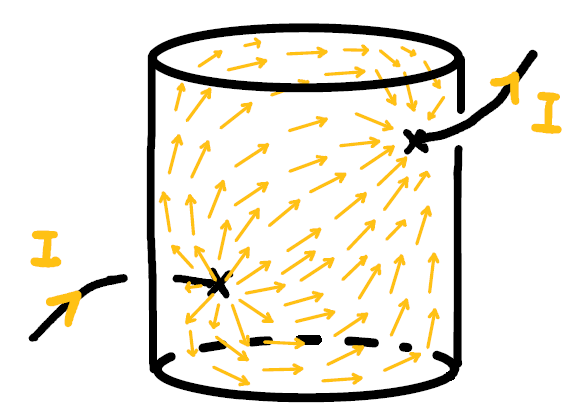
\includegraphics[height=8em]{current_vol}
    \end{minipage}
\end{center}

\vskip 1em
\begin{notation}[Caution:]
    In magneto\cul[red]{statics} problem, we require the current flow to be \cul[red]{independent of time}.
    Although you may have learnt that a moving point charge $q$ traveling at velocity $v$ acts like a point current source $qv$,
    we do not consider this as a static case because \cul[red]{this current is time-varying}.

    \begin{center}
        \begin{minipage}{0.48\linewidth}
            \centering
            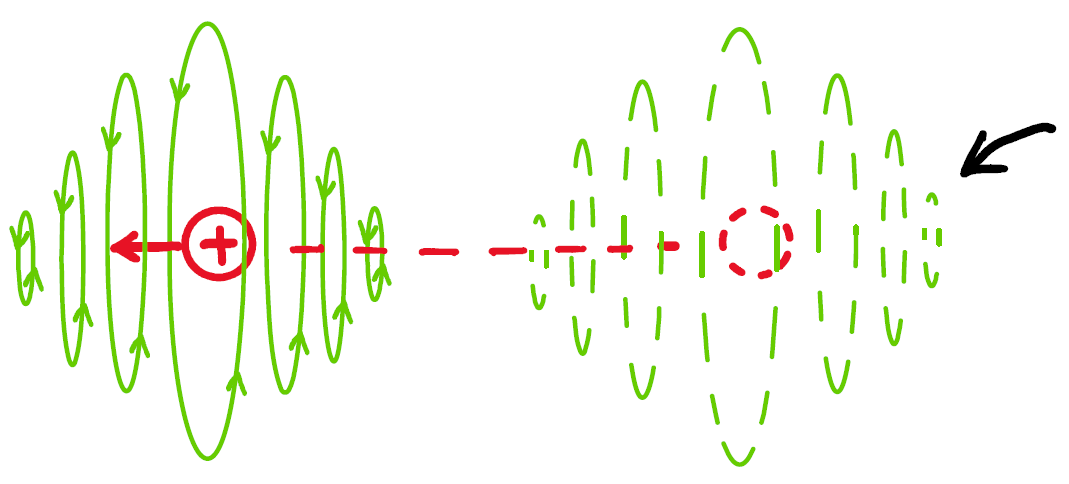
\includegraphics[width=\textwidth]{current_charge}
        \end{minipage}
        \begin{minipage}{0.4\linewidth}
            \centering
            The B-field here is created\\
            \bf{only for a short duration}.\\
            This B-field is NOT static.\\
            And neither is the current created by point charge.
        \end{minipage}
    \end{center}

    Moreover, the true formula of B-field by point charge needs to consider the travelling time of B-field (light speed).
    But this is completely out of our scope.

\end{notation}

\newpage
\begin{example}
    Suppose there is a wire lying on the x-axis, 
    with its ends at $x=a$ and $x=b$.
    Let there be uniform current $I$ flowing along it.
    What is the B-field on an arbituary point on the z axis?
    \begin{center}
        \begin{minipage}{0.3\linewidth}
            \centering
            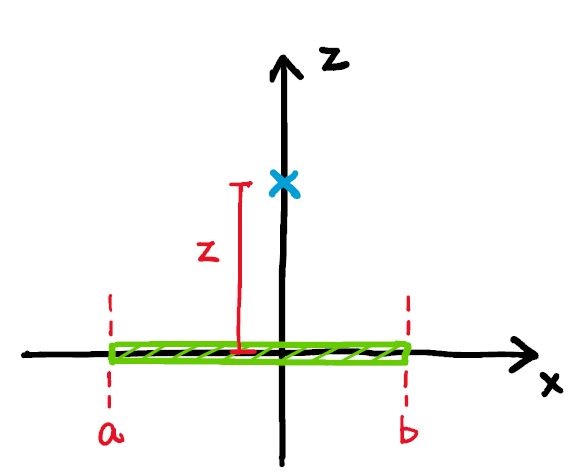
\includegraphics[width=\textwidth]{rod1}
        \end{minipage}
        \hspace{0.1\textwidth}
        \begin{minipage}{0.3\linewidth}
            \centering
            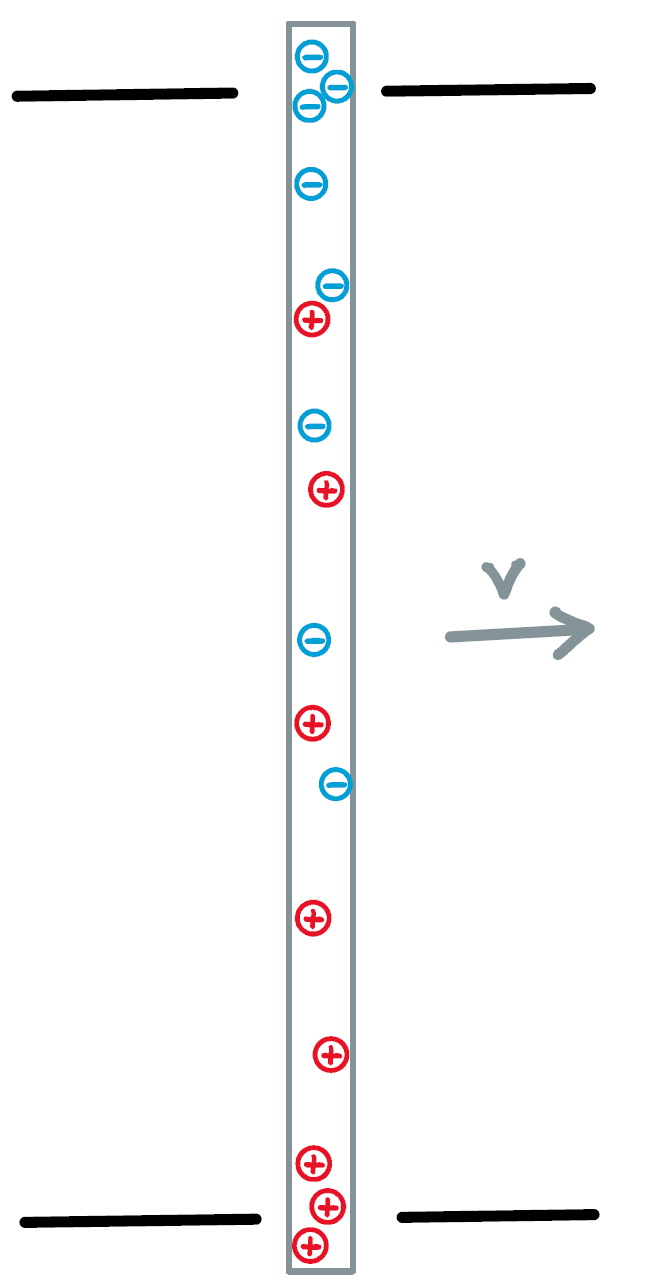
\includegraphics[width=\textwidth]{rod2}
        \end{minipage}
    \end{center}

    We can analyze by dividing the rod into infinitestimal pieces:
    \begin{itemize}
        \item Each segment has a length $\dd{x}$
        \item Each unit of current segment is thus $I\dd{\vvec{x}} = I\dd{x}\hhat{x}$.
        \item For the segment at position $x$, 
        its distance from the targeted point is $\sqrt{z^2+x^2}$.
    \end{itemize}

    Thus we can calculate $\vvec{B}$ by Biot-Savat law.
    \aleq{
        \vvec{B} = \frac{\mu_0}{4\pi}\int_a^b \frac{I\dd{x}\hhat{x}}{z^2+x^2}\cross \qty(\substack{\text{directon to}\\\text{target point}})
    }
    To do the cross product, 
    we need to resolve the direction's component from the segment to the target point. 

    \begin{minipage}{0.5\linewidth}
        \aleq{
            \hhat{r} &= \frac{x}{\sqrt{z^2+x^2}}\hhat{x} + \frac{z}{\sqrt{z^2+x^2}}\hhat{z}\\
            \Rightarrow\quad \hhat{x}\cross\hhat{r} &= \frac{z}{\sqrt{z^2+x^2}}(-\hhat{y})
        }
    \end{minipage}
    \hspace{0.05\textwidth}
    \begin{minipage}{0.15\linewidth}
        \centering
        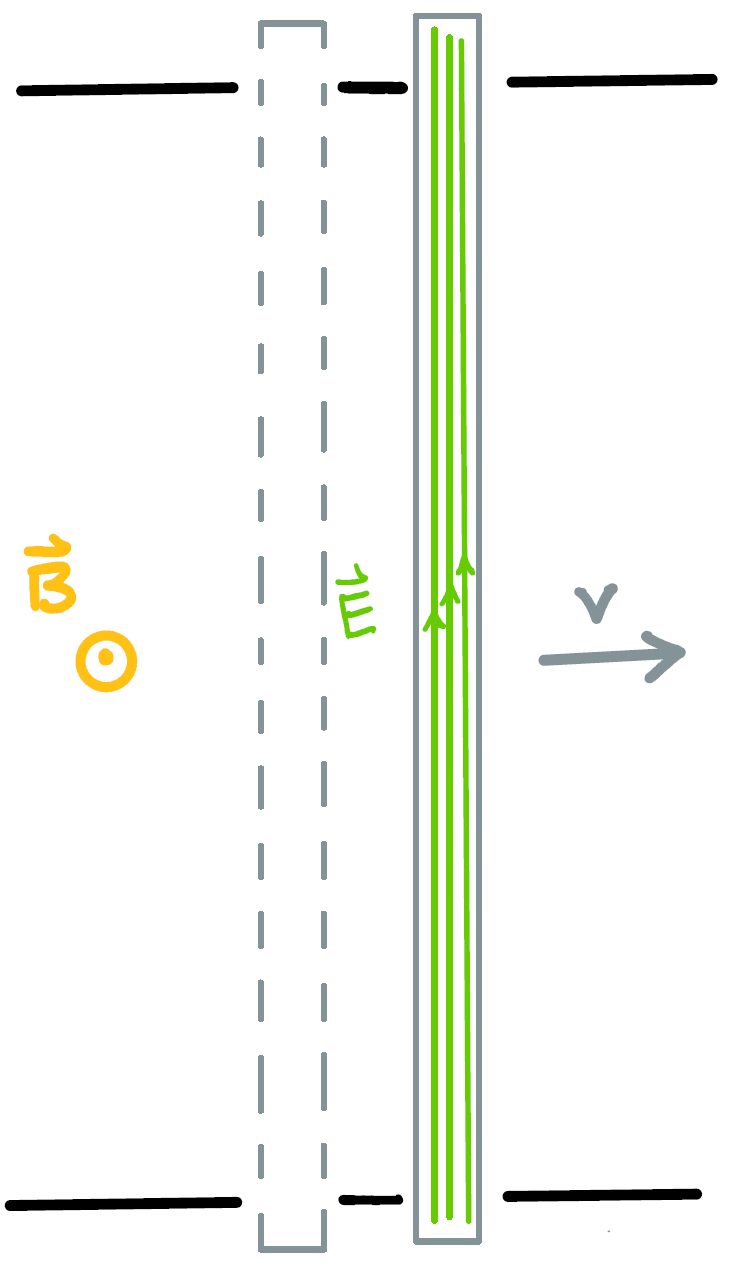
\includegraphics[width=\textwidth]{rod3}
    \end{minipage}

    \vskip 1em
    In this situation, $-\hhat{y}$ is the out of paper direction. 

    \begin{center}
        \begin{minipage}{0.18\linewidth}
            \centering
            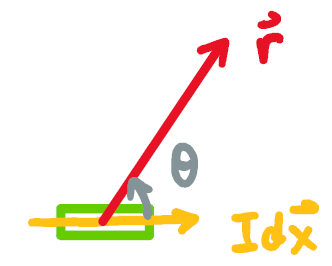
\includegraphics[width=\textwidth]{rod4}
        \end{minipage}
        \hspace{0.1\textwidth}
        \begin{minipage}{0.18\linewidth}
            \centering
            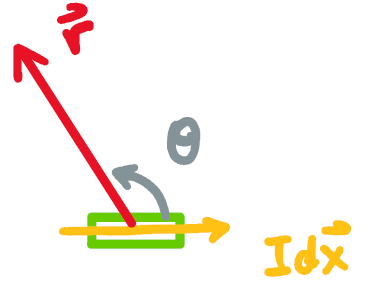
\includegraphics[width=\textwidth]{rod5}
        \end{minipage}
        \hspace{0.05\textwidth}
        \begin{minipage}{0.45\linewidth}
            \centering
            You can also deduce by cross product $\vvec{B} \sim I\dd{\vvec{x}} \cross \hhat{r}$ -
            line elements on both sides of the rod create a B-field in out-of-paper ($-\hhat{y}$)direction.  
        \end{minipage}
    \end{center}

    So the result B-field should be integrated as
    \aleq{
        B_y = - \frac{\mu_0}{4\pi}\int_a^b \frac{I\dd{x}}{z^2+x^2}\frac{z}{\sqrt{z^2+x^2}}
    }


\end{example}


\linesep
% Section %%%%%%%%%%%%%%%%%%%%%%%%%%%%%%%%%%%%%%%%%%%%%%%%%%%%
\section{Divergent-less of B-field}

Similar to E-field, there is the \bf{Gauss's law for B-field},
which has two different expressions: 
\aleq{
    \oiint \vvec{B}\cdot \dd{\vvec{s}} &= 0 &(\text{Integral form})\\[1ex]
    %
    \div \vvec{B} &= 0 &(\text{Differential form})
}

This law is purely an observation to B-field, claiming that 
\aleq{
    \Aboxed{
        \mstack{\text{Magnetic point source}\\[0.5ex]\text{does not exist}}
        \qquad\Leftrightarrow\qquad
        \mstack{\text{Total flux of B-field}\\[0.5ex]\text{on a closed surface always}= 0}
    }
}

Because so far no one has found any magnetic monopoles,
we determine that B-field lines must exist as closed loops,
and can never form diverging/converging patterns like E-field does.\\

This law is not as important as the other 3 in the Maxwell equation because 
it does not involve any source terms.
It is only sometimes useful when we need to make symmetry claims or simplify derivations.



\linesep
% Section %%%%%%%%%%%%%%%%%%%%%%%%%%%%%%%%%%%%%%%%%%%%%%%%%%%%
\section{Ampere's Law}

The Ampere's Law (in magnetostatics) has two different expressions:
\aleq{
    \oint \vvec{B}\cdot \dd{\vvec{l}} &= \mu_0 I &(\text{Integral form})\\[1ex]
    %
    \curl \vvec{B} &= \mu_0 \vvec{J} &(\text{Differential form})
}

It is easier to study the physical meaning and visualize by the integral form.
After that we can generalize to the differential form by introducing an operator called \bf{curl}.

%%%%%%%%%%%%%%
\subsection{Revisit: Dot Product Line Integral}

The literal description in Ampere's law integral form is
\aleq{
    \qty(\mstack{\text{Dot product line integral}\\\text{of magnetic field along a loop}})
    \ =\ \oint \vvec{B}\cdot \dd{\vvec{l}}
    \ =\ \mu_0 I
    \ =\ (\text{Constant})(\text{Current enclosed})
}

Recall that we can use the sign of a dot product between 2 vectors to 
determine if the vectors are in similar / opposite directions. 

\begin{center}
    \begin{minipage}{0.27\linewidth}
        \centering
        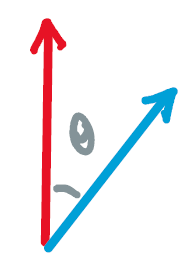
\includegraphics[width=0.25\textwidth]{dot1}\\[2ex]
        If $\vvec{a}\cdot\vvec{b}>0$,\\
        $\vvec{a}$ and $\vvec{b}$ are 
        more or less in similar directions.
    \end{minipage}
    \quad\vline\quad
    \begin{minipage}{0.28\linewidth}
        \centering
        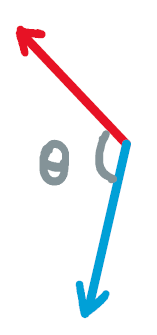
\includegraphics[width=0.2\textwidth]{dot2}\\
        If $\vvec{a}\cdot\vvec{b}<0$,\\
        $\vvec{a}$ and $\vvec{b}$ are 
        more or less in opposite directions.
    \end{minipage}
    \quad\vline\quad
    \begin{minipage}{0.30\linewidth}
        \centering
        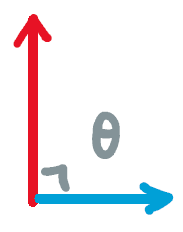
\includegraphics[width=0.25\textwidth]{dot3}\\[1.5ex]
        If $\vvec{a}\cdot\vvec{b}=0$,\\
        $\vvec{a}$ and $\vvec{b}$ are 
        perpendicular to each other.
    \end{minipage}
\end{center}

Now consider that we are travelling in a vector field along some path.
At each step, 
we can take note of field vector there and our travelling direction,
then compute their dot product.

\begin{center}
    \begin{minipage}{0.45\linewidth}
        \centering
        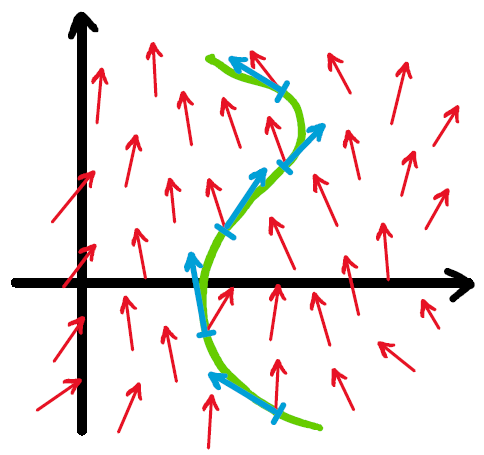
\includegraphics[width=0.6\textwidth]{dot4}\\
        If the total of all the dot products $>0$,\\ 
        we are travelling around the same direction as the field's flow.
    \end{minipage}
    \quad\vline\quad
    \begin{minipage}{0.45\linewidth}
        \centering
        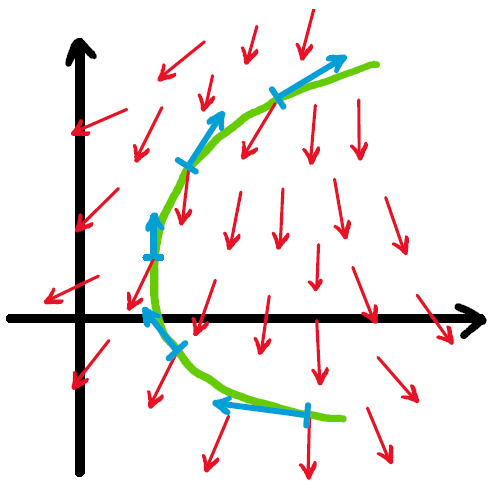
\includegraphics[width=0.6\textwidth]{dot5}\\
        If the total of all the dot products $<0$,\\
        we are travelling around the opposite direction as the field's flow.
    \end{minipage}
\end{center}

\vskip 1em
If we divide our path into infinitestimal small segments,
then the sum become line integral.
\aleq{
    \int_\text{path} \vvec{F}\cdot \dd{l}
    \quad
    \begin{cases}
        > 0 &\Rightarrow\quad \sim \text{Our path is along the flow}\\
        < 0 &\Rightarrow\quad \sim \text{Our path is opposite to the flow}
    \end{cases}
}


%%%%%%%%%%%%%%
\subsection{Detection of Rotating Flow}

The situation becomes interesting if we choose our path to be a closed loop - 
this loop integral becomes an indicator whether there are rotation trends around the loop.\\

By convention, we \red{always use an anti-clockwise loop} (Just like right hand rule). 

\begin{center}
    \begin{minipage}{0.5\linewidth}
        \centering
        If $\displaystyle \oint_{\substack{\text{our}\\\text{loop}}} \vvec{F}\cdot \dd{l} > 0$,
        the loop may have enclosed some rotation centers of anti-clockwise flow.
    \end{minipage}
    \hspace{0.05\textwidth}
    \begin{minipage}{0.25\linewidth}
        \centering
        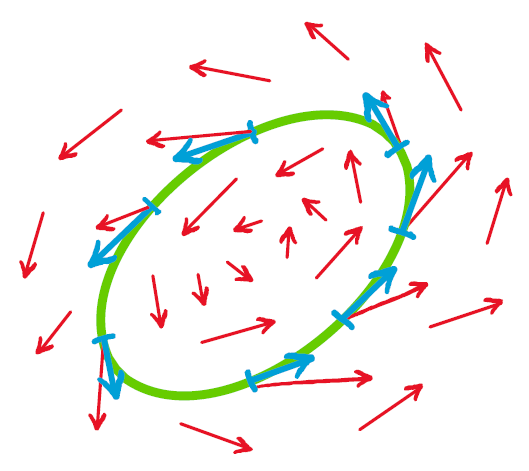
\includegraphics[height=8em]{dot_loop1}
    \end{minipage}
\end{center}
\begin{center}
    \begin{minipage}{0.5\linewidth}
        \centering
        If $\displaystyle \oint_{\substack{\text{our}\\\text{loop}}} \vvec{F}\cdot \dd{l} < 0$,
        the loop may have enclosed some rotation centers of clockwise flow.
    \end{minipage}
    \hspace{0.05\textwidth}
    \begin{minipage}{0.25\linewidth}
        \centering
        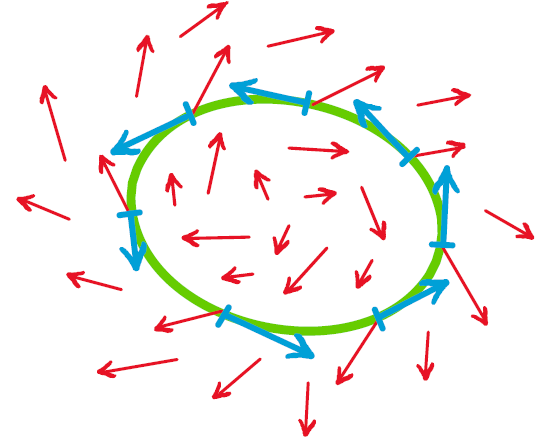
\includegraphics[height=8em]{dot_loop2}
    \end{minipage}
\end{center}
\begin{center}
    \begin{minipage}{0.5\linewidth}
        \centering
        If $\displaystyle \oint_{\substack{\text{our}\\\text{loop}}} \vvec{F}\cdot \dd{l} \approx 0$,
        the loop probably does not enclose any rotation centers.
    \end{minipage}
    \hspace{0.05\textwidth}
    \begin{minipage}{0.25\linewidth}
        \centering
        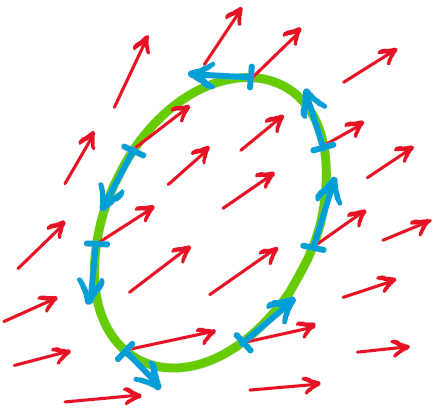
\includegraphics[height=8em]{dot_loop3}
    \end{minipage}
\end{center}




%%%%%%%%%%%%%%
\subsection{Curl}

However there is a problem in using loop integral of dot product - 
if we choose the loop too arbituarily, 
the calculated dot product is ambiguous to tell where the rotation centers are.
\begin{center}
    \begin{minipage}{0.2\linewidth}
        \centering
        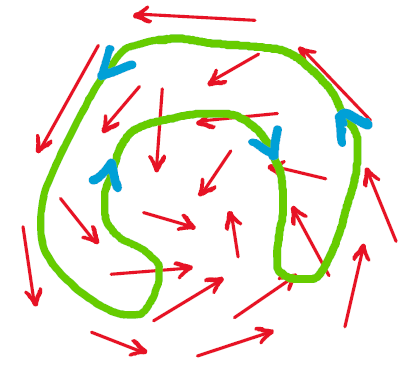
\includegraphics[width=\textwidth]{dot_loop4}
    \end{minipage}
    \hspace{0.1\textwidth}
    \begin{minipage}{0.35\linewidth}
        \centering
        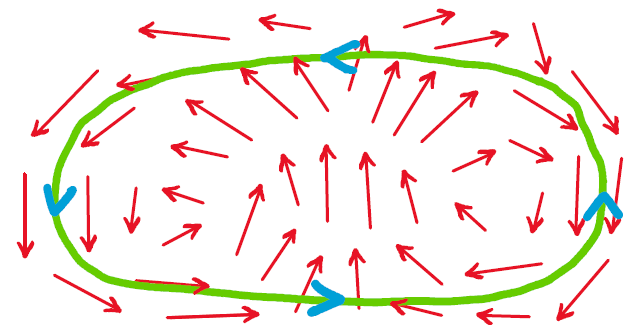
\includegraphics[width=\textwidth]{dot_loop5}
    \end{minipage}
\end{center}

E.g. If we choose an irregular loop, it may not catch the positions of rotation centers.\\

To tackle this problem,
we need to introduce the \bf{curl} operator:
\aleq{
    \tkn{curl}{\cul[red]{\curl}}\ \bullet 
    \ \defeq\ \curlRec{\bullet_x}[\bullet_y][\bullet_z]
    \ \defeq\ \tkn{curl2}{\cul[blue]{\text{curl}}}\ \bullet
}
\addArrow[red]{curl}{(0,-3ex)}
{\scriptsize Like gradient operator\\[-1ex]\scriptsize but with a cross}
{(0,-1ex)}{(0,-1ex)}
\addArrow[blue]{curl2}{(0,-3ex)}
{\scriptsize Sometimes we\\[-1ex]\scriptsize just write "curl"}
{(0,-1ex)}{(0,-1ex)}


\vskip 1em
The curl operator can be applied on a vector function,
and it returns another vector function.
\aleq{
    \curl{F} 
    &= \bmat{\pdvv{x} & \pdvv{y} & \pdvv{z}}\cross \bmat{F_x & F_y & F_z}\\[1ex]
    &= \curlRecDet{F_x}[F_y][F_z]\\[1ex]
    &= \curlRec{F_x}[F_y][F_z]\\[1ex]
    &= (\text{A vector})
}

Each component of the curl of a vector field is related to its
\bf{loop integral along an infinitestimal small loop in each direction.}


%%%%%%%%%%%%%%
\subsubsection{Geometrical Interpretation}

To visualize, we can draw 3 infinitestimal small loop around a point $(x,y,z)$.
Because of symmetry in all 3 directions,
it suffices to just analyze the loop that is parallel to the $x$-$y$ plane.

\begin{center}
    \begin{minipage}{0.4\linewidth}
        \centering
        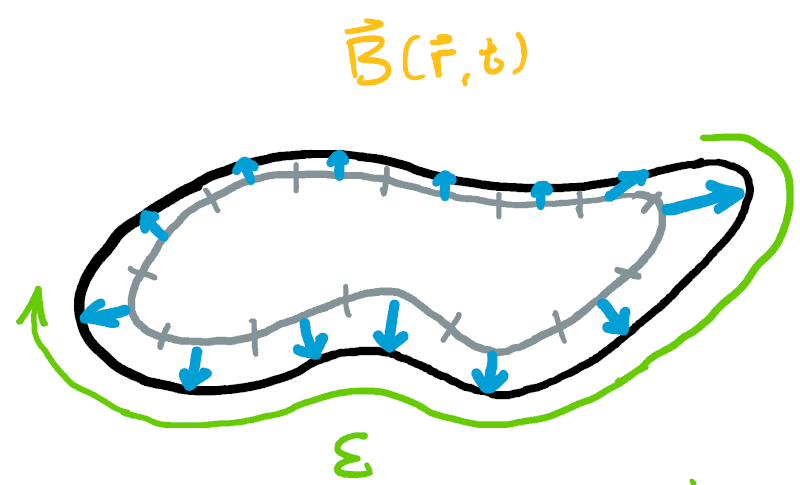
\includegraphics[width=\textwidth]{loop1}
    \end{minipage}
    {\large \quad$\Rightarrow$\qquad}
    \begin{minipage}{0.15\linewidth}
        \centering
        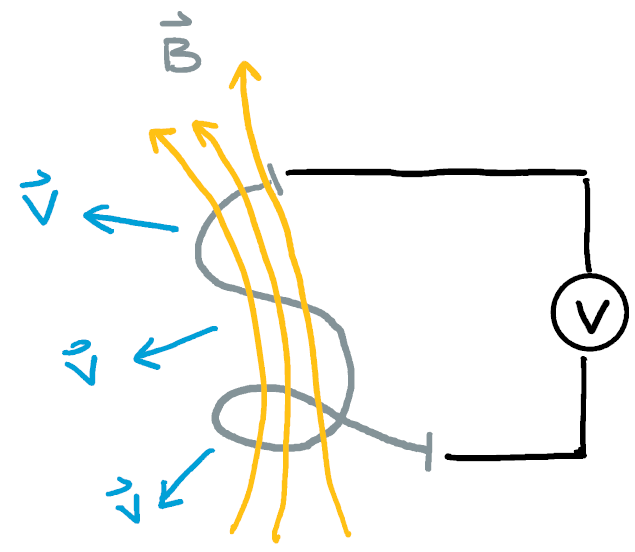
\includegraphics[width=\textwidth]{loop2}
    \end{minipage}
\end{center}

The dot product on each side of the loop are calculated as follow:

\begin{center}
    \begin{minipage}{0.6\linewidth}
        \centering
        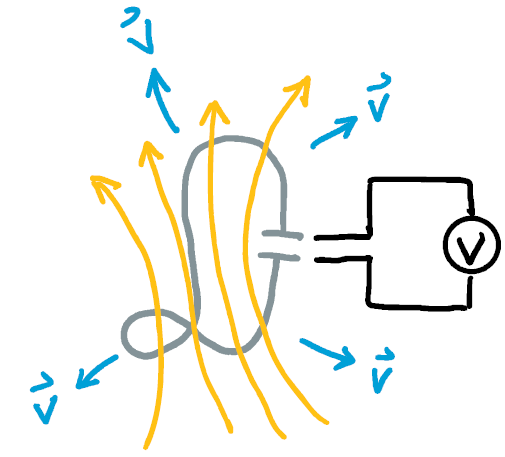
\includegraphics[width=\textwidth]{loop3}
    \end{minipage}
\end{center}


\vskip 1em
\begin{itemize}
    \item \ul{Edge 1} :\\[1ex]
    \begin{minipage}{0.8\linewidth}
        \begin{itemize}
            \item Vector field on the edge center = \red{$\vvec{F}\qty(x,y+\frac{\Delta y}{2},z)$}
            \item Edge length = \blue{$\Delta x$}, in $-x$ direction
        \end{itemize}
        $\Rightarrow\ \qty(\text{Dot product}) = \vvec{F}\qty(x,y+\frac{\Delta y}{2},z)\cdot (\Delta x)(-\hhat{x})
        = -F_{\cul[blue]{\cul[blue]{x}}}\qty(x,y+\frac{\Delta y}{2},z)\Delta x$

    \end{minipage}
    \hspace{0.02\textwidth}
    \begin{minipage}{0.18\linewidth}
        \centering
        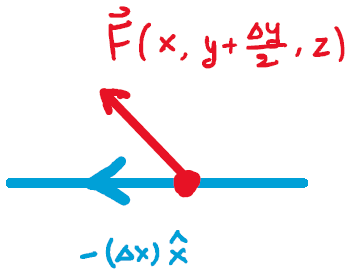
\includegraphics[width=\textwidth]{loop_e1}
    \end{minipage}

    
    \vskip 1em
    \item \ul{Edge 2} :\\[1ex]
    \begin{minipage}{0.8\linewidth}
        \begin{itemize}
            \item Vector field on the edge center = \red{$\vvec{F}\qty(x-\frac{\Delta x}{2},y,z)$}
            \item Edge length = \blue{$\Delta y$}, in $-y$ direction
        \end{itemize}
        $\Rightarrow\ \qty(\text{Dot product}) = \vvec{F}\qty(x-\frac{\Delta x}{2},y,z)\cdot (\Delta y)(-\hhat{y})
        = -F_{\cul[blue]{\cul[blue]{y}}}\qty(x-\frac{\Delta x}{2},y,z)\Delta y$

    \end{minipage}
    \hspace{0.01\textwidth}
    \begin{minipage}{0.18\linewidth}
        \centering
        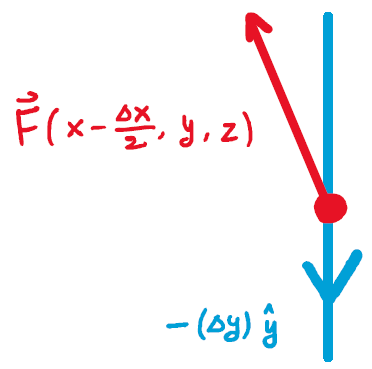
\includegraphics[width=\textwidth]{loop_e2}
    \end{minipage}
    

    \vskip 1em
    \item \ul{Edge 3} :\\[1ex]
    \begin{minipage}{0.8\linewidth}
        \begin{itemize}
            \item Vector field on the edge center = \red{$\vvec{F}\qty(x,y-\frac{\Delta y}{2},z)$}
            \item Edge length = \blue{$\Delta x$}, in $+x$ direction
        \end{itemize}
        $\Rightarrow\ \qty(\text{Dot product}) = \vvec{F}\qty(x,y-\frac{\Delta}{2},z)\cdot (\Delta x)(+\hhat{x})
        = F_{\cul[blue]{\cul[blue]{x}}}\qty(x,y-\frac{\Delta y}{2},z)\Delta x$

    \end{minipage}
    \hspace{0.02\textwidth}
    \begin{minipage}{0.18\linewidth}
        \centering
        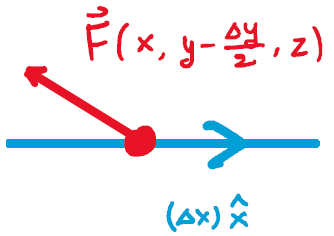
\includegraphics[width=\textwidth]{loop_e3}
    \end{minipage}

    \vskip 1em
    \item \ul{Edge 4} :\\[1ex]
    \begin{minipage}{0.8\linewidth}
        \begin{itemize}
            \item Vector field on the edge center = \red{$\vvec{F}\qty(x+\frac{\Delta x}{2},y,z)$}
            \item Edge length = \blue{$\Delta y$}, in $+y$ direction
        \end{itemize}
        $\Rightarrow\ \qty(\text{Dot product}) = \vvec{F}\qty(x+\frac{\Delta x}{2},y,z)\cdot (\Delta y)(+\hhat{y})
        = F_{\cul[blue]{\cul[blue]{y}}}\qty(x+\frac{\Delta x}{2},y,z)\Delta y$

    \end{minipage}
    \hspace{0.01\textwidth}
    \begin{minipage}{0.18\linewidth}
        \centering
        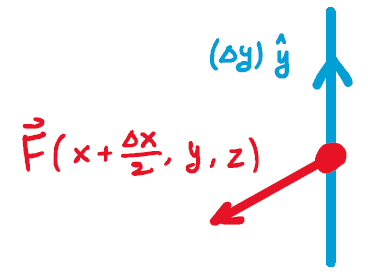
\includegraphics[width=1.05\textwidth]{loop_e4}
    \end{minipage}

\end{itemize}

Therefore the total dot product along the loop is
\aleq{
    &\textstyle \cus[gray]{F_y\qty(x+\frac{\Delta x}{2},y,z)\Delta y}{\text{Edge 4}} 
        - \cus[gray]{F_y\qty(x-\frac{\Delta x}{2},y,z)\Delta y}{\text{Edge 2}}
        - \cus[gray]{F_x\qty(x,y+\frac{\Delta y}{2},z)\Delta x}{\text{Edge 1}} 
        + \cus[gray]{F_x\qty(x,y-\frac{\Delta y}{2},z)\Delta x}{\text{Edge 3}} \\[1em]
    %
    = &\qty(\frac{F_x\qty(x+\frac{\Delta x}{2},y,z) - F_x\qty(x-\frac{\Delta x}{2},y,z)}{\blue{\Delta x}}
        - \frac{F_x\qty(x,y+\frac{\Delta y}{2},z) - F_x\qty(x,y-\frac{\Delta y}{2},z)}{\blue{\Delta y}}) (\Delta x\Delta y)\\[1em]
    %
    = &\qty(\cut[red]{\cbox[red]{\frac{F_x\qty(\cbox[red]{\textstyle x+\frac{\Delta x}{2}},y,z) 
            - F_x\qty(\cbox[red]{\textstyle x-\frac{\Delta x}{2}},y,z)}{\cbox[red]{\Delta x}}}}{\text{This is exactly partial x}}
        -\cut[green]{\cbox[green]{\frac{F_x\qty(x,\cbox[green]{\textstyle y+\frac{\Delta y}{2}},z) 
            - F_x\qty(x,\cbox[green]{\textstyle y-\frac{\Delta y}{2}},z)}{\cbox[green]{\Delta y}}}}{\text{This is exactly partial y}}) (\Delta x\Delta y)\\[1em] 
    %
    = &\qty(\pdvv{F_y}{x} - \pdvv{F_x}{y})(\Delta x\Delta y)\\[1em]
    %
    =& \qty(\mstack{\text{Curl's }\\[0.5ex] z\text{ component}})
        \qty(\mstack{\text{Unit area}\\[0.5ex]\text{parallel to xy plane}})\\[1em]
    %
    =& \qty(\mstack{\text{Curl's }\\[0.5ex] z\text{ component}})
        \qty(\mstack{\text{Unit area}\\[0.5ex]\text{\blue{normal to z direction}}})
}

\vskip 1em
We can expect the similar results in the other 2 directions.
Gather them together:
\aleq{
    \bcase{
        \qty(\mstack{\text{Loop integral}\\\text{normal to}\\[0.2ex]x \text{ direction}})
        = \qty(\pdvv{F_z}{y} - \pdvv{F_y}{z})(\dd{y}\dd{z})
        = (\curl \vvec{F})_x (\dd{y}\dd{z})
        = \qty(\mstack{\text{Curl's }\\[0.5ex] x\text{ component}})
            \qty(\mstack{\text{Unit area}\\[0.2ex]\text{normal to}\\[0.2ex]x \text{ direction}})\\[1em]
        %
        \qty(\mstack{\text{Loop integral}\\\text{normal to}\\[0.2ex]y \text{ direction}})
        = \qty(\pdvv{F_z}{x} - \pdvv{F_x}{z})(\dd{z}\dd{x})
        = (\curl \vvec{F})_y (\dd{z}\dd{x})
        = \qty(\mstack{\text{Curl's }\\[0.5ex] y\text{ component}})
            \qty(\mstack{\text{Unit area}\\[0.2ex]\text{normal to}\\[0.2ex]y \text{ direction}})\\[1em]
        %
        \qty(\mstack{\text{Loop integral}\\\\\text{normal to}\\[0.2ex]z \text{ direction}})
        = \qty(\pdvv{F_y}{x} - \pdvv{F_x}{y})(\dd{x}\dd{y})
        = (\curl \vvec{F})_z (\dd{x}\dd{y})
        = \qty(\mstack{\text{Curl's }\\[0.5ex] z\text{ component}})
            \qty(\mstack{\text{Unit area}\\[0.2ex]\text{normal to}\\[0.2ex]z \text{ direction}})\\[1em]
    }
}

\vskip 1ex
Therefore we can geometrically interpret curl as
\aleq{
    \Aboxed{
        \qty(\mstack{\text{\bf{Curl's}}\\\text{\bf{i\Nth\ component}}}) 
        = (\curl \vvec{F})_i 
        = \frac{(\text{Loop integral normal to i\Nth\ direction})}{(\text{Area enclosed by the loop})}
        \sim \qty(\mstack{\text{\bf{loop integral}}\\\tkn{curl_density}{\text{\bf{\cul[blue]{density}}}}})_\bf{\tkn{curl_dir}{\cul[red]{i}}}
    }
}
\addArrow[blue]{curl_density}{(0,-4ex)}{\scriptsize This density\\[-1ex]\scriptsize is by area}{(0,-1ex)}{(0,-1ex)}
\addArrow[red]{curl_dir}{(0,-3ex)}{\scriptsize In i\Nth\\[-1ex]\scriptsize direction}{(0,-0.5ex)}{(0,-1ex)}

\vskip 1em
%%%%%%%%%%%%%%
\subsubsection{Stokes' Theorem}

With the geometrical interpretation,
we can directly state (without proof) a convenient formula related to curl - 
the \bf{Stokes' theorem}:
\aleq{
    \Aboxed{
        \oint \vvec{F}\cdot \dd{\vvec{l}} &= \iint (\curl \vvec{F}) \cdot \dd{\vvec{s}}
    }
}

which is basically 
\aleq{
    \qty(\mstack{\text{Total }\\[0.5ex]\text{Loop integral}})
    \quad \sim \sum_{\text{All area}} \qty(\mstack{\text{Loop integral}\\[0.5ex]\text{per area}})\times \qty(\text{Area})
}


%%%%%%%%%%%%%%
\subsection{Ampere's Law - Explanation}


The Ampere's law is purely an \cul[red]{observation} about the relation between B-field and currents:
\aleq{
    \Aboxed{
        \mstack{\text{Total line integral of B-field}\\[0.5ex]\text{along a closed loop}\neq 0}
        \qquad\Leftrightarrow\qquad
        \mstack{\text{There are currents}\\[0.5ex]\text{circled by the loop}}
    }
}

The two forms of Ampere's law are describing this same observation:
\begin{itemize}
    \item \ul{Integral form}:
    \vskip -5ex
    \aleq{
        (\vvec{B}\text{'s loop integral})\ \sim\ \oint \vvec{B}\cdot\dd{\vvec{l}} 
        \ =\ \mu_0 I \ \sim\ (\text{Current})
    }

    \item \ul{Differential form}:
    \vskip -5ex
    \aleq{
        \qty(\mstack{\vvec{B} \text{'s loop integral}\\[0.5ex]\text{density}})\ \sim\ \curl \vvec{B}
        \ =\ \mu_0 \vvec{J}\ \sim\ \qty(\mstack{\text{Current}\\[0.5ex]\text{density}})
    }
\end{itemize}

And the two form can be inter-converted by Stokes' theorem.
\addArrow[red]{curlB}{(0,9ex)}{Stokes' Theorem}{(1ex,3ex)}{(-10ex,-6ex)}
\addBentArrow[blue]{curlI}{(-3.5ex,11.5ex)}{Current to Current density}{(1ex,3ex)}{(18ex,-6ex)}
\aleq{
    \oint \vvec{B}\cdot\dd{\vvec{l}} \quad &=\quad \mu_0 I\\[2em]
    \iiint (\tkn{curlB}{\curl \vvec{B}}) \cdot \dd{\vvec{s}}\ &=\ \mu_0\iint \tkn{curlI}{\vvec{J}} \cdot \dd{\vvec{s}}
}


%%%%%%%%%%%%%%
\subsection{Applying Ampere's Law Integral Form}

In beginner electromagnetism, 
there is only one type of problems related to Ampere's law: 
\quoting{
    Given the current distribution, 
    find the B-field everywhere by Ampere's law integral form\\
    in some \cul[red]{very symmetrical} scenarios.
}
which is basically asking you to \it{revert} the loop integral calculation:
\aleq{
    \oint \vvec{B}\cdot\dd{\vvec{l}} = \mu_0 I
    \qquad\Rightarrow\qquad
    \vvec{B} = \text{Some function of }I
}

If $I$ has a very ugly distribution, 
there is nothing we can do other than solving some PDEs.
But \red{if $I$ distributes very symmetrically, 
$\vvec{B}$ should also be symmetrical}, 
such that the loop integral can be broken into multiplications.\\

In these cases, we can choose an "Amperian" loop to to be integrated where
\begin{enumerate}
    \item $\vvec{B}$ has constant magnitude everywhere along the loop.
    \item $\vvec{B}$ forms the same angle with the tangent vector everywhere along the loop.
\end{enumerate}

\vskip 1ex
Only then, the loop integral can be broken down as
\aleq{
    \oint \vvec{B}\cdot \dd{\vvec{l}} 
    &= \oint \tkn{ampere_dot}{\cul[green]{\norm{\vvec{B}}\norm{\dd{\vvec{l}}}\cos\theta}}\\[1ex]
    &= \tkn{ampere_B}{\cul[red]{\norm{\vvec{B}}}}\ \tkn{ampere_theta}{\cul[blue]{\cos\theta}}\ \oiint \norm{\dd{\vvec{l}}}\\[2.5em]
    &= \norm{\vvec{B}}\ \cos\theta\ (\text{Perimeter of loop})
}
\addArrow[green]{ampere_dot}{(5ex,0)}
{\scriptsize Just dot product\\[-1ex]\scriptsize $\vvec{a}\cdot\vvec{b}=\norm{\vvec{a}}\norm{\vvec{b}}\cos\theta$}
{(8ex,0)}{(6ex,0)}
\addBentArrow[red]{ampere_B}{(-8ex,-3.5ex)}
{Same magnitude everywhere\\[-0.5ex]Can move out of integral!}
{(0,-1.5ex)}{(-12.5ex,1ex)}
\addBentArrow[blue]{ampere_theta}{(8ex,-3.5ex)}
{Form same angle everywhere\\[-0.5ex]Can move out of integral!}
{(0,-1.5ex)}{(12.5ex,1ex)}

such that we can find the magnitude of $\vvec{B}$ with simple division
\aleq{
    \Aboxed{
        \norm{\vvec{B}} 
        = \frac{(\text{Total loop integral})}{(\text{Perimeter of loop})\cos\theta}
        = \frac{\mu_0 I}{(\text{Perimeter of loop})\cos\theta}
    }
}

In fact, there are not many of these "very symmetrical" cases.
These examples below, with their respective Amperian loops,
are basically all the variations you can find in textbooks.

\begin{center}
    \begin{tabular}{>{\centering\arraybackslash}m{0.3\linewidth}
        >{\centering\arraybackslash}m{0.3\linewidth}
        >{\centering\arraybackslash}m{0.3\linewidth}}
        \makecell{Current configuration\\(Assuming uniform density)} 
        & & Good Amperian loop 
        \\[1ex]
        \hline
        Infinitely long wire
        &
        \vskip 1ex
        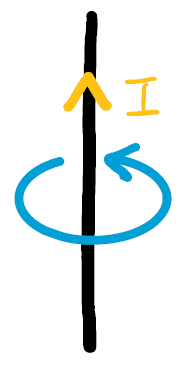
\includegraphics[width=0.25\linewidth]{wire}
        &
        \blue{Circle}
        \\[2ex]
        %
        Infinitely long solenoid
        &
        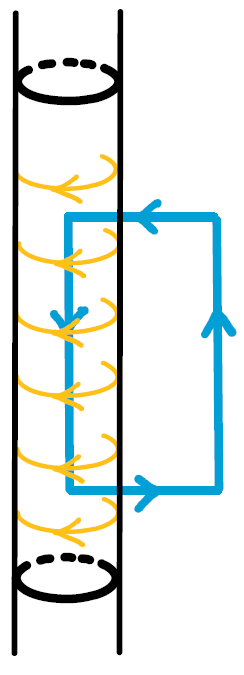
\includegraphics[width=0.3\linewidth]{solen}
        &
        \blue{Rectangle at cross-section}
        \\[1ex]
        %
        Infinitely large plane
        &
        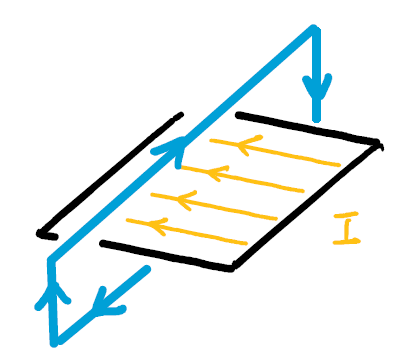
\includegraphics[width=0.6\linewidth]{plane}
        &
        \blue{Infinitely large rectangle wrapping it around}
        \\[3em]
        %
        Toroidal solenoid
        &
        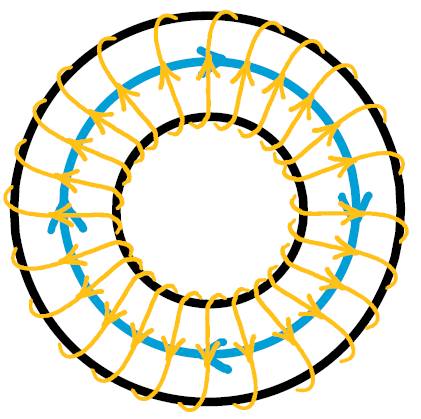
\includegraphics[width=0.6\linewidth]{torus}
        &
        \blue{Circle through center of the core}
    \end{tabular}
\end{center}

\begin{example}
    Given an infinitely long wire with current $I$ flowing along.
    By cylindrical symmetry, the B-field must satisfy:

    \begin{minipage}{0.6\linewidth}
        \begin{itemize}
            \item Unchange when translate along the wire (z-axis).
            \item Unchange when rotate about the wire (z-axis).
        \end{itemize}
    \end{minipage}
    \begin{minipage}{0.15\linewidth}
        \centering
        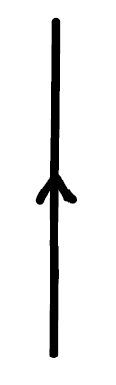
\includegraphics[height=6em]{wire2}
    \end{minipage}

    
    Note that cylindrical symmetry does not restrict the B-field to be circle loops.
    For example, all of these configurations satisfy cylindrical symmetry:

    \begin{center}
        \begin{minipage}{0.3\linewidth}
            \centering
            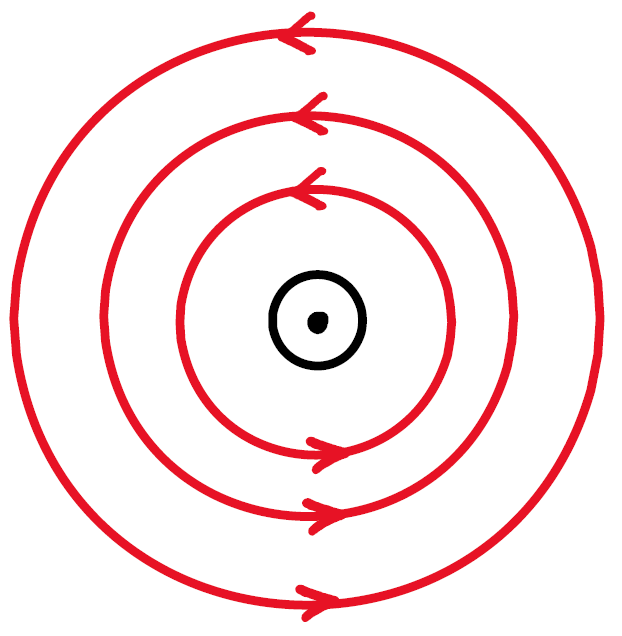
\includegraphics[height=8em]{wire_loop}\\
            If $\vvec{B}$ only has $\hhat{\theta}$ component\\
            $\Rightarrow$ Circular loops
        \end{minipage}
        \hspace{0.01\textwidth}
        \begin{minipage}{0.25\linewidth}
            \centering
            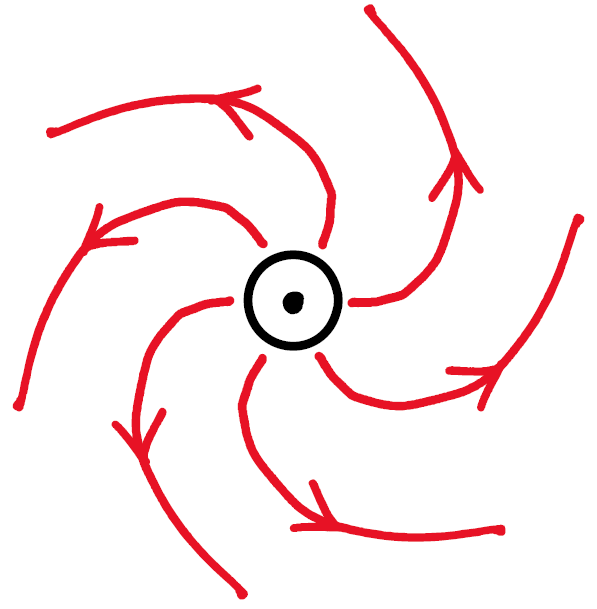
\includegraphics[height=8em]{wire_r}\\
            If $\vvec{B}$ has $\hhat{r}$ component\\
            $\Rightarrow$ Can spiral out
        \end{minipage}
        \hspace{0.01\textwidth}
        \begin{minipage}{0.25\linewidth}
            \centering
            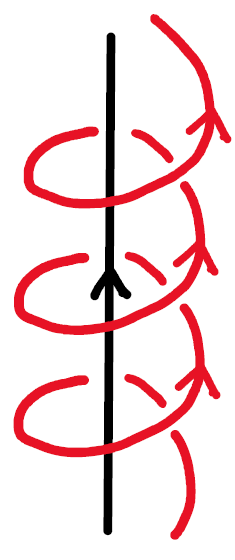
\includegraphics[height=8em]{wire_z}\\
            If $\vvec{B}$ has $\hhat{z}$ component\\
            $\Rightarrow$ Can spiral up
        \end{minipage}
    \end{center}

    We need to rule out the 2 latter cases before we can use Ampere's law to find $\vvec{B}$:\\

    \begin{minipage}{0.8\linewidth}
        \begin{enumerate}
            \item \ul{$\vvec{B}$ is divergent-less} : \\[1ex]
            We can draw a cylindrical Gaussian box around the wire.\\
            If the B-field has $\hhat{r}$ component,
            we would get the flux of $\vvec{B} \neq 0$.\\
            Then it contradicts to $\vvec{B}$ being divergent-less.
            
        \end{enumerate}
    \end{minipage}
    \hspace{0.05\textwidth}
    \begin{minipage}{0.1\linewidth}
        \centering
        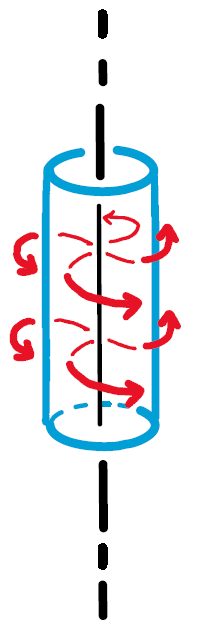
\includegraphics[height=9em]{wire_div}
    \end{minipage}
    
    \begin{enumerate}
        \item[2.] \ul{Another Amperian loop} : \\[1ex]
        We can draw an Amperian loop that is parallel to the wire.
        By Ampere's law, there is no current enclosed by this loop,
        so the loop integral should be $0$.

        \begin{center}
            \begin{minipage}{0.5\linewidth}
                \centering
                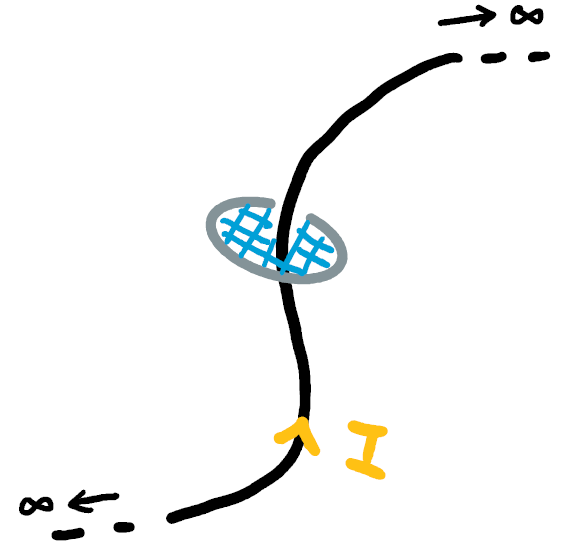
\includegraphics[width=\textwidth]{wire_inf}
            \end{minipage}
        \end{center}

        \begin{itemize}
            \item By translational symmetry, 
            the dot product at the top (edge 2) and bottom (edge 4) should cancel each other. 
            
            \vskip 1ex
            \item First choose the loop which stretches to infinitly far.
            Because there should be no B-field at infinity,
            dot product on edge 3 should be $0$.

            \vskip 1ex
            \item Then if we choose a loop which does not stretch to infinitly far,
            we can conclude that the dot product on edge 1 is $0$.
            So this $\vvec{B}$ must not have $\hhat{z}$ component.
        \end{itemize}
    \end{enumerate}

    After all these symmetry arguments,
    we can finally conclude that B-field around a wire must be circular loops. 
    We can choose a circular Amperian loop of radius $r$ to find the magnitude of B-field
    at distance $r$ from the wire.
    \aleq{
        \norm{\vvec{B}} 
        &= \frac{\mu_0 I}{(\text{Perimeter of loop})\cos\theta}\\
        &= \mu_0 I \cdot \inv{(2\pi r)} \cdot \inv{\cos \tkn{ampere_cylth}{\cul[green]{0^\circ}}}\\
        &= \frac{\mu_0 I}{2\pi r}\\[1ex]
        \Rightarrow\quad \vvec{B} &= \frac{\mu_0 I}{2\pi r} \tkn{ampere_cylph}{\cul[blue]{\hhat{\theta}}}
    }
    \addArrow[green]{ampere_cylth}{(7ex,0)}
    {\scriptsize B-field = angular \\[-1ex]\scriptsize $\therefore$ Tangent to loop}{(2ex,0.5ex)}{(5.5ex,1ex)}
    \addArrow[blue]{ampere_cylph}{(3ex,0)}
    {\scriptsize You have to manually add the unit vector}{(2ex,0.5ex)}{(15ex,0)}


\end{example}


\begin{example}
    Given an infinitely long solenoid made of a uniform density of coils $\frac{N}{L}$,
    with a current $I$ passiing through.
    This is another cylindrical symmetry case.\\

    \begin{minipage}{0.65\linewidth}
        \begin{itemize}
            \item Unchange when translate along the wire (z-axis).
            \item Unchange when rotate about the wire (z-axis).
        \end{itemize}

        Again, cylindrical symmetry does not restrict the B-field to be purely along z direction. 
        We need to first argue that the B-field does not have radial or angular components 
        before we can apply Ampere's law.

    \end{minipage}
    \hspace{0.05\textwidth}
    \begin{minipage}{0.25\linewidth}
        \centering
        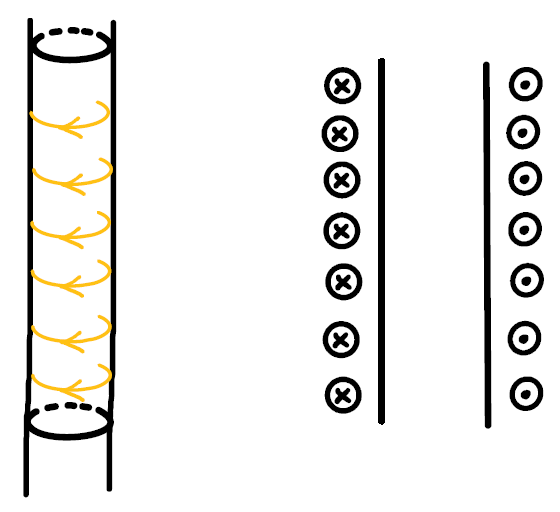
\includegraphics[width=\textwidth]{solen_cross}
    \end{minipage}
    
    \vskip 1em
    \begin{minipage}{0.72\linewidth}
        \begin{enumerate}
            \item \ul{$\vvec{B}$ is divergent-less} : \\[1ex]
            We can draw a cylindrical Gaussian box around the solenoid.\\
            If the B-field has $\hhat{r}$ component,
            we would get the flux of $\vvec{B}\neq 0$.\\
            Then it contradicts to $\vvec{B}$ being divergent-less.
                
        \end{enumerate}
    \end{minipage}
    \hspace{0.05\textwidth}
    \begin{minipage}{0.1\linewidth}
        \centering
        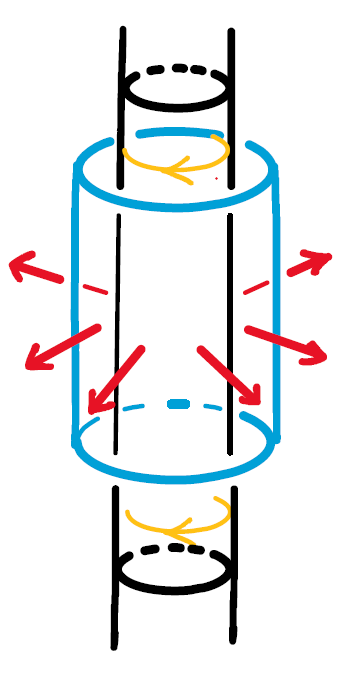
\includegraphics[height=9em]{solen_div}
    \end{minipage}

    \vskip 2em
    \begin{minipage}{0.72\linewidth}
        \begin{enumerate}
            \item[2.] \ul{Another Amperian loop} : \\[1ex]
            We can draw a loop that circulates around the solenoid.\\
            Because there is no current enclosed by this loop,\\
            dot product integral around this loop must be $0$.\\
            By Ampere's law, this B-field must not have $\hhat{\theta}$ component.
        \end{enumerate}
    \end{minipage}
    \hspace{0.05\textwidth}
    \begin{minipage}{0.1\linewidth}
        \centering
        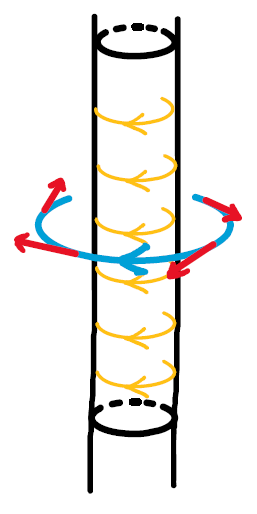
\includegraphics[height=9em]{solen_loop}
    \end{minipage}

    \vskip 2em
    Now we can conclude that B-field created by a solenoid must be in z direction only. 
    We can choose a circular Amperian loop over the cross-section of the solenoid,
    with one edge in the center of solenoid and another edge at infinitely far. 

    \begin{center}
        \begin{minipage}{0.6\linewidth}
            \centering
            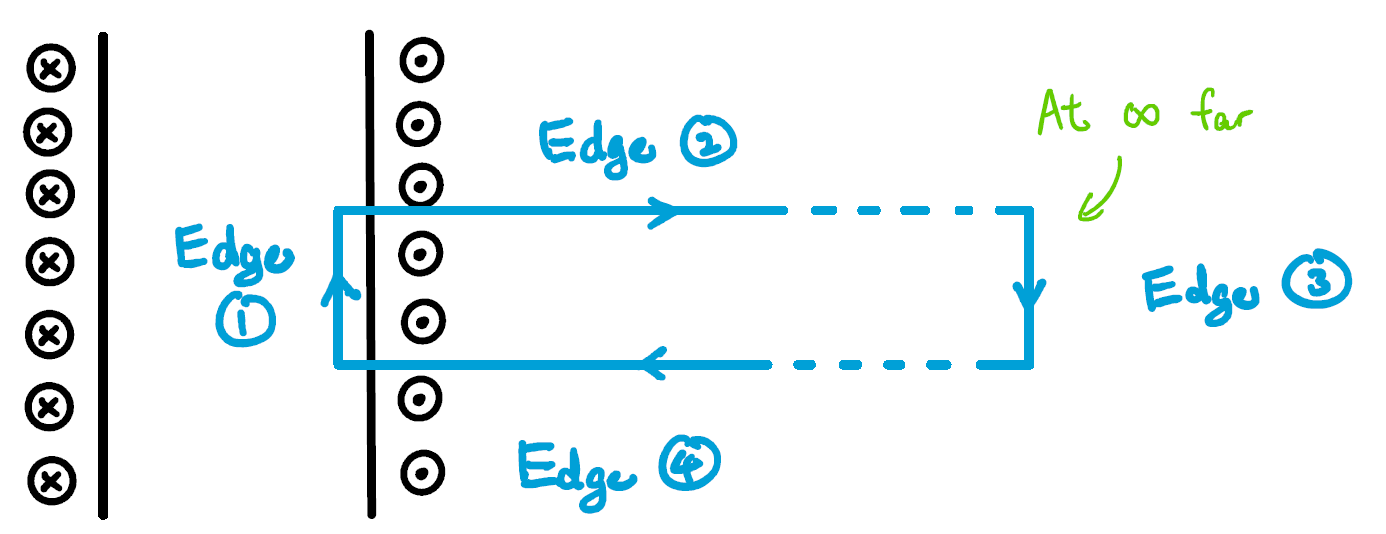
\includegraphics[width=\textwidth]{solen_inf}
        \end{minipage}
    \end{center}

    \begin{itemize}
        \item We have already argued that this B-field has no radial component.
        Dot product on edge 2 and 4 must be $0$.

        \item At infinitely far, there should be no B-field at infinity,
        dot product on edge 3 should be $0$.
    \end{itemize}

    So only edge 1 can have a non-zero dot product. 
    We can now apply Ampere's law:
    \aleq{
        \cub[gray]{\norm{\vvec{B}}L\cos{0^\circ}}{\text{Edge 1}}
        + \cub[gray]{0 + 0 + 0}{\text{Edge 2 \& 3 \& 4}}% + \cub[gray]{0}{\text{Edge 3}} + \cub[gray]{0}{\text{Edge 4}}
        &= \mu_0 (NI)\\
        %
        \norm{\vvec{B}} &= \frac{\mu_0 NI}{L}\\
        \vvec{B} &= \frac{\mu_0 NI}{L}\tkn{ampere_sol}{\cul[blue]{\hhat{z}}}
    }
    \addArrow[blue]{ampere_sol}{(3ex,0)}
    {\scriptsize You have to manually\\[-1ex]\scriptsize add the unit vector}
    {(2ex,0.5ex)}{(8ex,0)}

\end{example}






\linesep
% Section %%%%%%%%%%%%%%%%%%%%%%%%%%%%%%%%%%%%%%%%%%%%%%%%%%%%
\section{Magnetic Vector Potential}

%%%%%%%%%%%%%%
\subsection{Mathematical Origin}

Magnetic field also has a corresponding potential function $\vvec{A}(\vvec{r})$.
But unlike electric potential,
the magnetic potential is a vector function. 
The reason to create it is purely mathematical:
\begin{itemize}
    \item \ul{Observation}: 
    B-field always form loops because we have never observed any magnetic point source.
    $\Rightarrow$ B-field is divergent-less.

    \item \ul{Mathematical fact}: 
    Any divergent-less field can be expressed as the curl of some vector function (i.e. vector potential).
\end{itemize}

Therefore we can define a vector function $\vvec{A}(\vvec{r})$,
called \bf{magnetic vector potential}, such that 
\aleq{
    \Aboxed{
        \vvec{B}(\vvec{r}) = \curl \vvec{A}(\vvec{r})
    }
}

Unlike electric potential,
there is no reverse formula for reversely computing $\vvec{A}$ from $\vvec{B}$.

%%%%%%%%%%%%%%
\subsection{Poisson Equation}

If we substitute $\vvec{B} = \curl \vvec{A}$ into the Ampere's law differential form,
we arrive at a new equation: 
\addBentArrow[red]{curlcurl}{(-1ex,5ex)}
{\scriptsize $\curl(\curl \vvec{F}) \equiv \grad(\div \vvec{F}) - \laplacian \vvec{F}$\\[-0.5ex]\scriptsize is a vector calculus identity\\[-1ex]\scriptsize commonly used in derivations.}
{(0,3ex)}{(14ex,0)}
\addArrow[blue]{divA}{(10ex,-3ex)}
{\scriptsize We can CHOOSE $\div \vvec{A}=0$.\\[-1ex]\scriptsize This freedom is similar to electric potential\\[-1ex]
    \scriptsize where we can CHOOSE to add any constant to $V$.\\[-1ex]\scriptsize The formal reason is called "gauge freedom".}
{(0,-2.5ex)}{(14ex,0)}
\aleq{
    \mu_0 \vvec{J} &= \curl \vvec{B}\\
    &= \curl (\curl \vvec{A})\\[0.5ex]
    &= \grad\cub[blue]{(\tkn{divA}{\div \vvec{A}})}{} - \laplacian \tkn{curlcurl}{\vvec{A}}\\[0.5ex]
    &= -\laplacian \vvec{A}\\[1ex]
    \Aboxed{
        \laplacian \vvec{A}(\vvec{r}) &= -\mu_0\vvec{J}(\vvec{r})
    }
}

\vskip 1ex
This is again the \bf{Poisson equation}, 
the same PDE that we have encountered in electric potential 
($\laplacian V(\vvec{r}) = - \frac{\rho(\vvec{r})}{\epsilon_0}$).
But for magnetic potential,
because it is a vector function, 
this is actually 3 equations, one for each direction:
\aleq{
    &\laplacian \bmat{A_x \\ A_y \\ A_z} = -\mu_0 \bmat{J_x\\J_y\\J_z}
} 

\vskip 1ex
\cul[red]{It is the most fundamental relation between magnetic vector potential and current}.
Given any configurations of current or vector potential,
idealy we can find the other using this PDE.

\begin{itemize}
    \item \ul{$\vvec{A}(\vvec{r})$ to $\vvec{J}(\vvec{r})$} : 
    The Laplacian operator is just a sum of \nth{2} order derivatives. 
    (And we 
    \\ \phantom{\ul{$\vvec{J}(\vvec{r})$ to $\vvec{A}(\vvec{r})$} :}
    just need to do it 3 times). Relatively easy.

    \item \ul{$\vvec{J}(\vvec{r})$ to $\vvec{A}(\vvec{r})$} : 
    Need to solve the Poisson equation (for 3 times),
    which are \nth{2} order non-
    \\ \phantom{\ul{$\vvec{J}(\vvec{r})$ to $\vvec{A}(\vvec{r})$} :} homogeneous linear PDEs. Awful!
\end{itemize} 

Unfortunately in realistic problems,
it is more frequent to ask for $\vvec{A}(\vvec{r})$ from $\vvec{J}(\vvec{r})$,
because we can usually confine the current distribution in a small region 
by using very small test objects;
but for vector potential, it is always everywhere. 

\begin{center}
    \begin{minipage}{0.15\linewidth}
        \centering
        {\small It is easy to make $\vvec{J}=0$\\ in most places}
    \end{minipage}
    \begin{minipage}{0.27\linewidth}
        \centering
        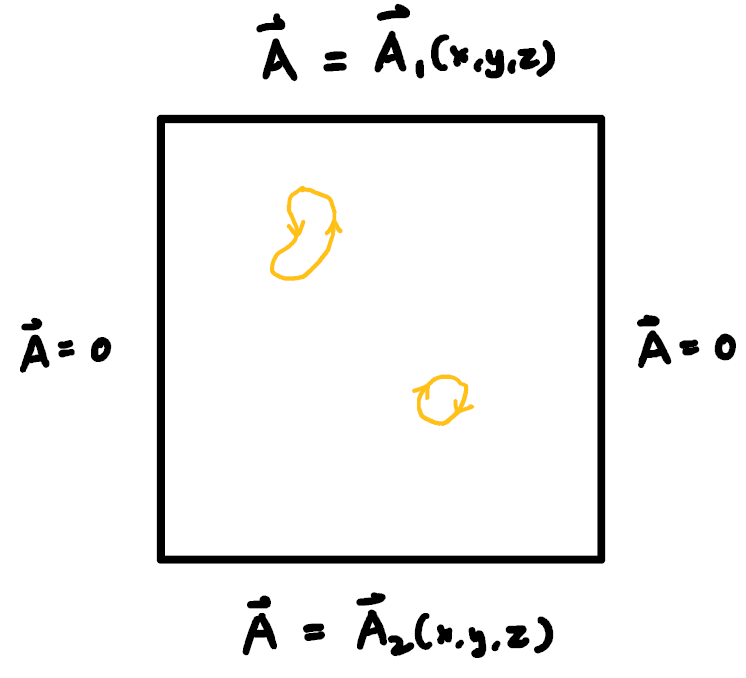
\includegraphics[width=\textwidth]{poisson_J}
    \end{minipage}
    {\Large \quad$\Leftrightarrow$\quad}
    \begin{minipage}{0.27\linewidth}
        \centering
        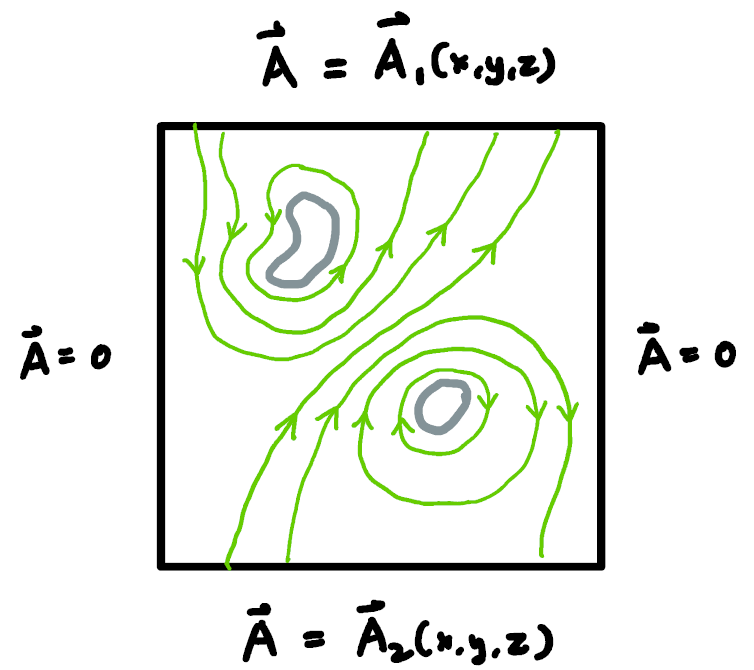
\includegraphics[width=\textwidth]{poisson_A}
    \end{minipage}
    \begin{minipage}{0.15\linewidth}
        \centering
        {\small It is difficult\\ to know $\vvec{A}$ everywhere}
    \end{minipage}
\end{center}

\newpage
Again we are not going to discuss how to solve it. 
Here I only provide you the solution in one very special case - 
When the \cul[red]{region of interest is infinitely large} + \cul[red]{$\vvec{A}$ is chosen to be divergent-less}, 
i.e. $\div \vvec{A}=0$, 
the solution is the Biot-Savat law for magnetic vector potential.

\begin{center}
    \begin{minipage}{0.4\linewidth}
        \aleq{
            \Aboxed{
                \vvec{A}(\red{\vvec{r}}) 
                &= \frac{\mu_0}{4\pi}\underset{\substack{\text{infinitely large}\\\text{space}}}{\iiint}\ 
                    \frac{\vvec{J}(\blue{\vvec{r}'})}{\norm{\red{\vvec{r}}-\blue{\vvec{r}'}}}\dd[3]{\blue{\vvec{r}'}}
            }\\[1ex]
            %
            &\sim \frac{\mu_0}{4\pi} \sum_\text{everywhere} \frac{(\text{current})}{(\text{distance})}\\[1em]
            %
            &\equiv\ \mstack{\text{Biot-Savat law for magnetic vector potential}\\\scriptsize \text{(written in a fancy vector form)}}
        }
    \end{minipage}
    \hspace{0.05\textwidth}
    \begin{minipage}{0.25\linewidth}
        \centering
        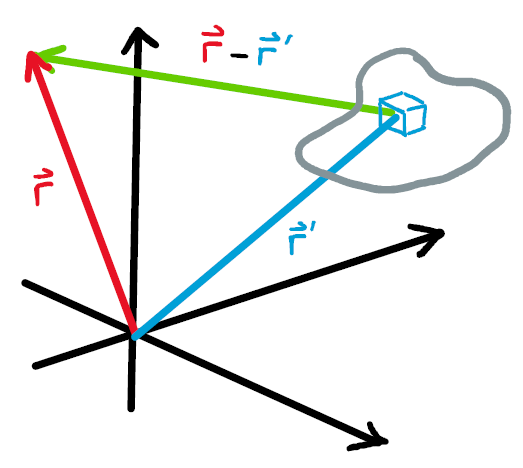
\includegraphics[width=\textwidth]{coulomb_elem}
    \end{minipage}
\end{center}





\vskip 1em
%%%%%%%%%%%%%%
\subsection{Finding $\vvec{B}$ from $\vvec{J}$}

On the other hand, Poisson equation provides an alternative to calculate B-field distribution from current distribution.
If we compare the Ampere's law and Poisson equation of $\vvec{A}$:
\begin{itemize}
    \item \ul{Poisson equation} : \\[1ex]
    Although $\vvec{A}(\vvec{r})$ is a vector function,
    the Poisson equations for each compoenent $A_x(\vvec{r})$, $A_y(\vvec{r})$, $A_z(\vvec{r})$ 
    are \cul[red]{independent}.
    \addArrow[red]{Jx}{(3ex,0)}{\scriptsize Only involve\\[-1ex]\scriptsize x components}{(2.5ex,0.5ex)}{(5ex,0)}
    \addArrow[red]{Jy}{(3ex,0)}{\scriptsize Only involve\\[-1ex]\scriptsize y components}{(2.5ex,0.5ex)}{(5ex,0)}
    \addArrow[red]{Jz}{(3ex,0)}{\scriptsize Only involve\\[-1ex]\scriptsize z components}{(2.5ex,0.5ex)}{(5ex,0)}
    \aleq{
        \laplacian \vvec{A} = -\mu_0 \vvec{J}
        \qquad\Leftrightarrow\qquad
        \bcase{
            \qty(\lapRec{})A_{\cul[red]{x}} &= -\mu_0 \tkn{Jx}{J_{\cul[red]{x}}}\\[1ex]
            \qty(\lapRec{})A_{\cul[red]{y}} &= -\mu_0 \tkn{Jy}{J_{\cul[red]{y}}}\\[1ex]
            \qty(\lapRec{})A_{\cul[red]{z}} &= -\mu_0 \tkn{Jz}{J_{\cul[red]{z}}}
        }
        \qquad
    }
    

    \item \ul{Ampere's law} :\\[1ex]
    $\vvec{B}(\vvec{r})$ is a vector function with 3 components $B_x(\vvec{r})$, $B_y(\vvec{r})$, $B_z(\vvec{r})$,
    Because of the curl operation, 
    the PDE for each component of $\vvec{B}$ and $\vvec{J}$ all mix together.
    \aleq{
        \curl \vvec{B} = \mu_0 \vvec{J}
        \qquad\Leftrightarrow\qquad
        \bcase{
            \curlPla[y][z]{B_z}[B_y] &= \mu_0 J_x\\[1ex]
            \curlPla[z][x]{B_x}[B_z] &= \mu_0 J_y\\[1ex]
            \curlPla[x][y]{B_y}[B_z] &= \mu_0 J_z\\[1ex]
        }
    }

\end{itemize}

In practice, there is no reason to try to directly solve the more difficult PDEs of $\vvec{B}$,
if we can alternatively solve the easier PDEs of $\vvec{A}$,
and then take curl to get $\vvec{B}$ (i.e. via $\vvec{B} = -\curl \vvec{A}$). 

\begin{center}
    \begin{minipage}{0.5\linewidth}
        \centering
        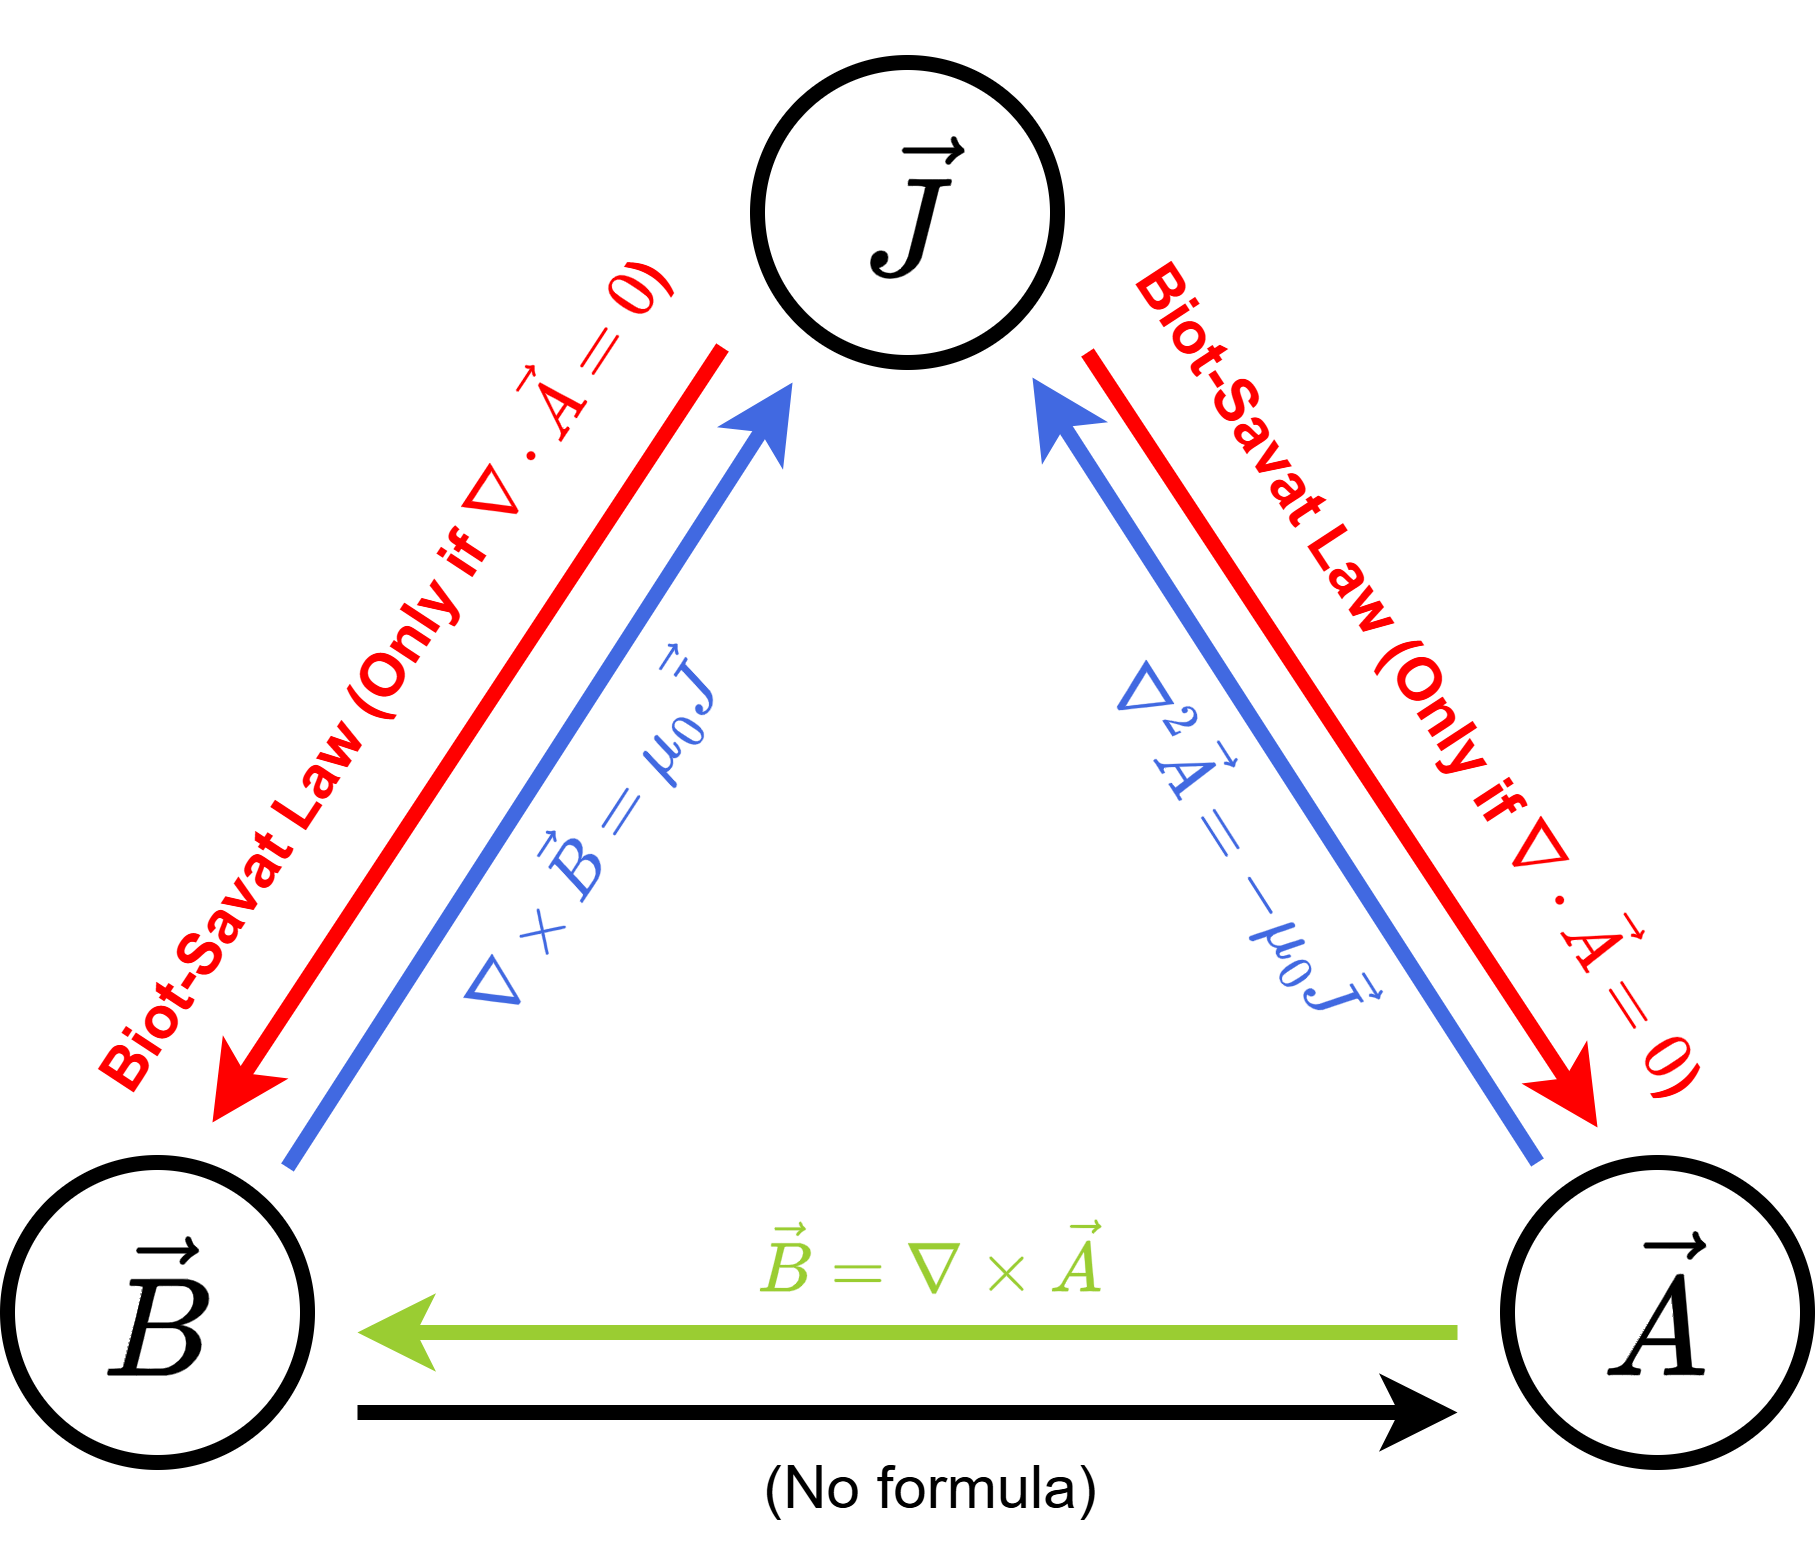
\includegraphics[width=\textwidth]{triangleB}
    \end{minipage}
\end{center}

In this way, we can tell the solution of Ampere's law as a PDE, 
which is as expected, the Biot-Savat law for $\vvec{B}$.
\aleq{
    \Aboxed{
        \vvec{B}(\red{\vvec{r}}) = \curl \vvec{A}(\red{\vvec{r}}) 
        &= \frac{\mu_0}{4\pi}\underset{\substack{\text{infinitely large}\\\text{space}}}{\iiint}\ 
            \frac{\vvec{J}(\blue{\vvec{r}'})}{\norm{\red{\vvec{r}}-\blue{\vvec{r}'}}^2}
            \cross\qty[\frac{\red{\vvec{r}}-\blue{\vvec{r}'}}{\norm{\red{\vvec{r}}-\blue{\vvec{r}'}}}]\dd[3]{\blue{\vvec{r}'}}
    }\\[1ex]
    %
    &\sim \frac{\mu_0}{4\pi} \sum_\text{everywhere} \frac{(\text{current})}{(\text{distance})^2} \cross \qty(\substack{\text{unit}\\\text{vector}})\\[1em]
    %
    &\equiv\ \mstack{\text{Biot-Savat law for magnetic field}\\\scriptsize \text{(But written in a fancier vector form)}}
}

\vskip 1em
\begin{notation}[Side note:]

    We have learnt 3 differential operator related to $\grad$. 
    \begin{itemize}
        \item \ul{Gradient} $\grad f$ \ -\ \  Scalar function $\xRightarrow{\grad}$ Vector function\\[-1.5em]
        \item \ul{Divergence} $\div \vvec{F}$ \ -\ \  Vector function $\xRightarrow{\div}$ Scalar function\\[-1.5em]
        \item \ul{Curl} $\curl \vvec{F}$ \ -\ \  Vector function $\xRightarrow{\curl}$ Vector function
    \end{itemize}
    We can derive several \nth{2} derivatives relations of $\grad$ (by brute force):
    \begin{itemize}
        \item \ul{Wrapped by gradient}: \\[-3ex]
        \aleq{
            \grad (\div \vvec{F}) &= %\qty(\gradRec{})\qty(\divRec{F_x}[F_y][F_z]) \\[0.5ex]
            \pdv{x}\qty(\pdv{F_x}{x} + \pdv{F_y}{y} + \pdv{F_z}{z})\hhat{x} 
                + \pdv{y}\qty(\pdv{F_x}{x} + \pdv{F_y}{y} + \pdv{F_z}{z})\hhat{y}\\[0.5ex]
                &\qquad + \pdv{z}\qty(\pdv{F_x}{x} + \pdv{F_y}{y} + \pdv{F_z}{z} )\hhat{z}
        }
        Cannot simplify further than this form.
    \end{itemize}
\end{notation}
\begin{notation}[]
    \begin{itemize}
        \item \ul{Wrapped by divergence}:
        \aleq{
            \div (\grad f) &\ \defeq\ \laplacian f \ =\  \lapRec{f} \qquad {\scriptsize \text{(Laplacian operator)}}\\[1ex]
            %
            \div (\curl \vvec{F}) &\ \equiv\ 0 \qquad \red{\scriptsize \text{(Divergence of curl is always 0)}}
        }

        \item \ul{Wrapped by curl}:
        \aleq{
            \curl (\grad f) &\ \equiv\ 0 \qquad \red{\scriptsize \text{(Curl of gradient is always 0)}}\\[1ex]
            %
            \curl (\curl \vvec{F}) &\ \equiv\ \ \grad (\div \vvec{F}) - \laplacian \vvec{F} \qquad {\scriptsize \text{(A useful identity)}}
        }
    \end{itemize} 

    \vskip 1ex
    The two "$\equiv 0$" relations are the reasons why we can have potential functions.
    \begin{enumerate}
        \item In electrostatics, $\vvec{E}$ is conservative $\Rightarrow$ Loop integral $=0$.
        Then by Stoke's law,
        \aleq{
            \oint_{\substack{\text{ANY}\\\text{loop}}} \vvec{E} \cdot \dd{\vvec{l}} 
            = \iint_{\substack{\text{ANY}\\\text{surface}}} (\curl \vvec{E})\cdot\dd{\vvec{s}} = 0 
            \quad\Rightarrow\quad 
            \curl \vvec{E} = 0
        }
        Because \red{curl of gradient is always 0}, 
        we can always replace $\vvec{E}$ with the gradient of some scalar function.
        \aleq{
            \curl \vvec{E} = 0 \quad\Rightarrow\quad \curl (\grad V) = 0
        }

        \item Divergence of $\vvec{B}$ is always 0,
        meanwhile \red{divergence of curl is always 0}. 
        So we can always replace $\vvec{B}$ with the curl of some vector function.
        \aleq{
            \div \vvec{B} = 0 \quad\Rightarrow\quad \div (\curl \vvec{A}) = 0
        }
    \end{enumerate}
\end{notation}

\iffalse
\begin{notation}[Side note 1:]
    We can verify the identity 
    $\curl (\curl \vvec{F}) \equiv \grad (\div \vvec{F}) - \laplacian \vvec{F}$ by brute force.
    \aleq{
        \grad (\div \vvec{F}) &= \qty(\gradRec{})\qty(\divRec{F_x}[F_y][F_z]) \\[1ex]
        %
        &= \qty(\pdv[2]{F_x}{x} + \pdv{F_y}{x}{y} + \pdv{F_z}{x}{z})\hhat{x}
        + \qty(\pdv{F_x}{y}{x} + \pdv[2]{F_y}{y} + \pdv{F_z}{y}{z})\hhat{y}
        + \qty(\pdv{F_x}{z}{x} + \pdv{F_y}{z}{y} + \pdv[2]{F_z}{z} )\hhat{z}\\[2ex]
        %
        \laplacian \vvec{F} &= \qty(\lapRec{F_x})\hhat{x} 
            + \qty(\lapRec{F_y})\hhat{y} 
            + \qty(\lapRec{F_z})\hhat{z} 
    }

    Combining together, 
    \aleq{
        \grad (\div \vvec{F}) - \laplacian \vvec{F} 
        &= 
        \biggl[
            \pdv{y}\cub[blue]{\qty(\pdv{F_y}{x} -\pdv{F_x}{y})}{\text{z component of }\curl \vvec{F}} 
            - \pdv{z}\cub[blue]{\qty(\pdv{F_x}{z} -\pdv{F_z}{x})}{\text{y component of }\curl \vvec{F}}
        \biggr]\hhat{x}\\[1ex] %
        &\quad\ + \biggl[
            \pdv{x}\cub[blue]{\qty(\pdv{F_y}{x} -\pdv{F_x}{y})}{\text{z component of }\curl \vvec{F}} 
            + \pdv{z}\cub[blue]{\qty(\pdv{F_z}{y} -\pdv{F_y}{z})}{\text{x component of }\curl \vvec{F}}
        \biggr]\hhat{y}\\[1ex] %
        &\quad\ + \biggl[
            \pdv{x}\cub[blue]{\qty(\pdv{F_x}{z} -\pdv{F_z}{x})}{\text{y component of }\curl \vvec{F}} 
            + \pdv{y}\cub[blue]{\qty(\pdv{F_z}{y} -\pdv{F_y}{z})}{\text{x component of }\curl \vvec{F}}
        \biggr]\hhat{z}\\[1ex]
        %
        &= \curl (\curl \vvec{F})
    }
\end{notation}
\fi

\linesep
%%%%%%%%%%%%%%
Here we shall summarize the methods of solving magnetostatics problems:
\begin{enumerate}
    \item Very symmetric configurations 
    $\Rightarrow$ Ampere's law integral form. No calculus required.

    \item Not so symmetric but satisfies $\div \vvec{A}=0$ 
    $\Rightarrow$ Multiple integral with Biot-Savat law.

    \item All the above do not apply 
    $\Rightarrow$ Solve Poisson equation explicitly. PDE hell. %\emoji{skull}.
\end{enumerate}
\linesep
%%%
\theend
\end{document}